\documentclass{article} 
\usepackage{tikz} 
\begin{document} 
\begin{center} 
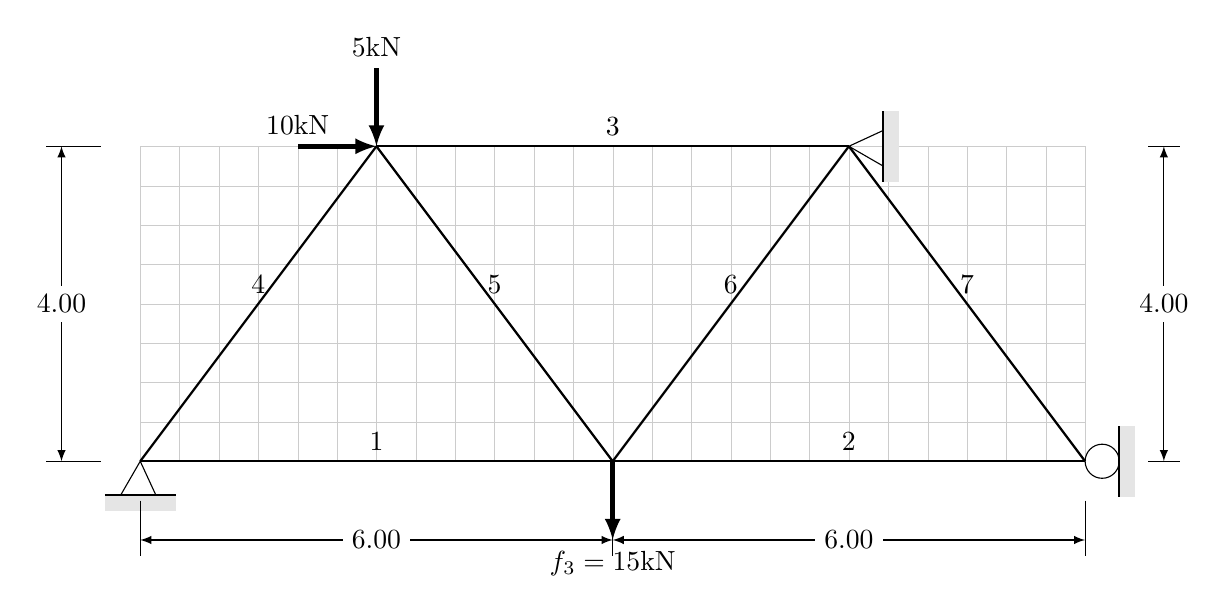
\begin{tikzpicture}[scale=1]

% definiciones

% estilos de linea y relleno
\tikzstyle{carga}   = [ultra thick,latex-]

% apoyo de segundo genero
\newcommand{\apoyoseg}[2]{
	\coordinate (O) at #1; % ubicación del apoyo
	\begin{scope}[rotate around={#2:(O)}]
	\fill [black!10](O) ++(-0.45,-0.433013) rectangle ++(0.9,-0.2);
	\draw [thick] (O) ++(-0.45,-0.433013) -- ++(0.9,0);
	\draw (O) -- ++(-0.25,-0.433013) -- ++(0.45,0) -- cycle;
	\end{scope}
}
% apoyo de primer genero
\newcommand{\apoyopri}[2]{
	\coordinate (O) at #1; % ubicación del apoyo
	\begin{scope}[rotate around={#2:(O)}]
	\fill [black!10](O) ++(-0.45,-0.433013) rectangle ++(0.9,-0.2);
	\draw [thick] (O) ++(-0.45,-0.433013) -- ++(0.9,0);
	\draw (O) ++(0,-0.216506) circle (0.216506);
	\end{scope}
}
% carga puntual
% #1: ubicación de la carga
% #2: rótulo de la carga
% #3=1: carga positiva, #3=-1: carga negativa
% #4=1,#5=0: carga en x, #4=0,#5=1: carga en y
% #6=0: carga entrando al nudo, #6=1: carga saliendo del nudo
% #7: ubicación del rótulo de la carga
\newcommand{\cargapun}[7]{
	\path #1 ++(#6*#4,#6*#5) coordinate (O);
	\draw [carga] (O) -- ++(-1.0*#3*#4,-1.0*#3*#5) 
	node [#7] {#2};
}

% cota horizontal
% #1: coordenada punto inicial ()
% #2: coordenada punto final ()
% #3: rotulo de la cota
% #4: separación entre puntos y cota
% #5: separación entre puntos y inicio de marcas
% #6: separación entre cota y fin de marcas
\newcommand{\cotahori}[6]{
\path #1 ++(0,#4) coordinate (A);
\path #2 ++(0,#4) coordinate (B);
\draw [latex-latex] (A) -- (B)
node [midway,fill=white] {#3};
\path #1 ++(0,#5) coordinate (C);
\path #1 ++(0,#4+#6) coordinate (D);
\draw (C) -- (D);
\path #2 ++(0,#5) coordinate (C);
\path #2 ++(0,#4+#6) coordinate (D);
\draw (C) -- (D);
}

% cota vertical
% #1: coordenada punto inicial ()
% #2: coordenada punto final ()
% #3: rotulo de la cota
% #4: separación entre puntos y cota
% #5: separación entre puntos y inicio de marcas
% #6: separación entre cota y fin de marcas
\newcommand{\cotavert}[6]{
	\path #1 ++(#4,0) coordinate (A);
	\path #2 ++(#4,0) coordinate (B);
	\draw [latex-latex] (A) -- (B)
	node [midway,fill=white] {#3};
	\path #1 ++(#5,0) coordinate (C);
	\path #1 ++(#4+#6,0) coordinate (D);
	\draw (C) -- (D);
	\path #2 ++(#5,0) coordinate (C);
	\path #2 ++(#4+#6,0) coordinate (D);
	\draw (C) -- (D);
}

% activar cuadrícula
\draw[step=0.5,black!20,ultra thin] (0,0) grid (12,4);
 
% elementos
\tikzstyle{elem}=[draw=black,thick];
\tikzstyle{nudo}=[midway,above];
\begin{scope}[elem]
\draw (0.000000,0.000000)--(6.000000,0.000000) node[nudo] {1}; 
\draw (6.000000,0.000000)--(12.000000,0.000000) node[nudo] {2}; 
\draw (3.000000,4.000000)--(9.000000,4.000000) node[midway,above] {3}; 
\draw (0.000000,0.000000)--(3.000000,4.000000) node[nudo] {4}; 
\draw (3.000000,4.000000)--(6.000000,0.000000) node[nudo] {5}; 
\draw (6.000000,0.000000)--(9.000000,4.000000) node[nudo] {6}; 
\draw (12.000000,0.000000)--(9.000000,4.000000) node[nudo] {7};
\end{scope} 

% apoyos y cargas
\apoyoseg{(0,0)}{0}
\apoyoseg{(9,4)}{90}
\apoyopri{(12,0)}{90}
\cargapun{(3,4)}{10kN}{1}{1}{0}{0}{above}
\cargapun{(3,4)}{5kN}{-1}{0}{1}{0}{above}
\cargapun{(6,0)}{$f_3=15$kN}{-1}{0}{1}{-1}{at start,below}

% cotas
\cotahori{(0,0)}{(6,0)}{6.00}{-1}{-0.5}{-0.2}
\cotahori{(6,0)}{(12,0)}{6.00}{-1}{-0.5}{-0.2}
\cotavert{(0,0)}{(0,4)}{4.00}{-1}{-0.5}{-0.2}
\cotavert{(12,0)}{(12,4)}{4.00}{1}{0.8}{0.2}






 
\end{tikzpicture} 
\end{center} 
\end{document} 
